% paper.tex — v4：三臂对照（no-rail / prompt-only / full-rail）× T1 结构化规划 / T2 开放写作 / openpool-T 开放引用池写作 × 3 seeds
% 所有数字与 experiments/exp1/<arm>/<seed>/<task>/results.json、no-rail/E1/results.json、
%   openpool/<arm>/<seed>/results.json、openpool/summary_*.json、audit/results.json、cost/results.json 及 <arm>/summary_*.json 逐字勾稽（F03）
% 所有 \cite 均命中 references/ 池（17/17 online verified，F04；references_index.json 提供 bibkey 映射）
\documentclass[10pt,twocolumn]{article}
\usepackage[utf8]{inputenc}
\usepackage{times}
\usepackage[margin=1in]{geometry}
\usepackage{booktabs}
\usepackage{graphicx}
\usepackage{tikz}
\usetikzlibrary{patterns}
\usepackage{amsmath,amssymb}
\usepackage{hyperref}
\usepackage[round]{natbib}
\usepackage{caption}
\usepackage{enumitem}
\setlength{\tabcolsep}{4pt}
\newcommand{\fit}[1]{\resizebox{\columnwidth}{!}{#1}}  % 表格缩放进栏宽

\title{Do Validation Rails Curb LLM Research-Agent Fabrication?\\ A Controlled Context-Engineering Experiment}
\author{CCF Team\\ Huawei openJiuwen Competition}
\date{}

\begin{document}
\maketitle

\begin{abstract}
Large language model (LLM) research agents automate proposal writing, experiment planning, and paper drafting, yet their outputs are prone to \emph{fabrication}: citations to non-existent papers, numbers without a verifiable source, and claims of work that was never executed. Existing mitigations are mostly post-hoc detectors or architectural proposals without controlled multi-seed evidence. We treat process-level \emph{validation rails}---structural checks on plan, results, and citation contracts---as a context-engineering intervention and measure their causal effect on fabrication rates under a fixed pipeline. In a fully controlled three-arm design, we hold tasks, model, and seeds fixed and switch only the rail assembly: no-rail, prompt-only, and full-rail (F02 plan validation, F03 results cross-checking, F04 citation verification, with rejection-redo gating). We first run a from-scratch no-rail control on structured planning (T1) and confirm that, on a closed pre-verified pool, all arms are at floor (CFR=NFR=UCR=0). To escape this floor, we introduce an adversarial writing task (T3) that disables online verification and allows the model to rely on memory: no-rail exhibits fabrication rates up to CFR=0.0769 and NFR=0.1071, while full-rail reduces both to 0.0 in every seed. Single-gate ablations show that F04 alone eliminates citation fabrication but leaves NFR at 0.0312 in one seed, whereas F03-only and prompt-only also reach 0.0 on this task. The cost of rails is measurable but bounded. We report floor effects, small-sample caveats, and data-credibility disclosures, and corroborate the finding with an open-citation-pool replication and an independent audit.
\end{abstract}

\section{Introduction}
\label{sec:intro}

LLM research agents are being deployed for end-to-end scientific workflows---ideation, experiment planning, execution, and writing. A core trust problem is \emph{fabrication}: models emit well-formatted but non-existent references, numbers that cannot be traced to any source, and claims that certain experiments were run when no such artifacts exist. The problem is empirically large and well documented: large-scale audits of citation corpora quantify the volume of hallucinated references \citep{zhao2026wildhallucinations}, and cross-model studies show that citation hallucination is prompt- and context-induced rather than intrinsic to the model \citep{naser2026howllmscite}, with legal-domain studies confirming the pattern in specialized settings \citep{alrajeh2026legalcitations}.

Existing mitigations fall into three families, none of which provides a controlled causal answer. First, \emph{post-hoc detection}: CiteAudit \citep{shi2026citeaudit}, CiteTracer \citep{li2026citetracer}, and HALLMARK \citep{reizinger2026hallmark} screen generated manuscripts for fabricated citations, but they do not prevent fabrication, and verifier false-positive rates are a known deployment bottleneck \citep{banerjee2026failuremodes}. Second, \emph{architectural proposals}: HALO \citep{raduta2026halo} advocates a hallucination-free-by-construction layered design, and Theoria \citep{saldivar2026theoria} verifies reasoning through auditable state transitions; Prompt-to-Paper \citep{kamran2026prompttopaper} combines deterministic retrieval with real experiment execution, and PhantomFill \citep{usman2026phantomfill} shows that form-mandated fields drive fabrication. These proposals are argued from first principles rather than measured under controlled conditions. Third, \emph{correlational measurement}: evidence that context quality predicts hallucination resistance \citep{bousetouane2026context} establishes relevance but not intervention; TRACE \citep{zhao2026trace} attributes context errors for automated repair, and Deep Agentic Search \citep{rafieioskooei2026deepagentic} isolates sub-agent context while risking silent handoff failures. No prior work treats a \emph{validation rail}---a process-level verification contract---as the manipulated variable and measures fabrication rates causally across multiple seeds.

Our approach is deliberately simple: we take the existing research-pipeline skill as the experimental platform and switch only the rail assembly (no-rail / prompt-only / full-rail F02+F03+F04) while holding tasks, model, and seeds fixed. We define a family of automatically computable fabrication metrics that are isomorphic to the rail checks themselves---citation fabrication rate (CFR), numeric fabrication rate (NFR), and unexecuted-claim rate (UCR)---so that \emph{measurement is auditing}. This paper reports the full three-arm, two-task, three-seed comparison. Our contributions are:

\begin{itemize}
\item We formalize CFR/NFR/UCR as reproducible, automatically computable fabrication metrics coupled to verification contracts (Section~\ref{sec:method}).
\item We run a controlled three-arm comparison---no-rail, prompt-only, full-rail---over structured planning (T1), open-domain writing (T2), and an adversarial writing task (T3), with three fixed seeds and metrics drawn verbatim from \texttt{experiments/exp1/*/results.json} (Section~\ref{sec:exp}).
\item We report a from-scratch clean no-rail T1 control that reaches floor (CFR=NFR=UCR=0), replacing the previously reconstructed E1 snapshot as the primary control (Section~\ref{sec:repro}).
\item We add a single-gate ablation: F02-only on T1, and F03-only/F04-only/prompt-only on the adversarial T3, isolating the contribution of each rail (Section~\ref{sec:ablation}, Section~\ref{sec:t3}).
\item In the adversarial T3 task, no-rail produces fabrication (CFR up to 0.0769, NFR up to 0.1071) while full-rail reduces both to 0.0 in all seeds; F04-only leaves a residual NFR in one seed, showing the need for combined gates (Section~\ref{sec:t3}).
\item We document rail gating behavior and disclose floor effects, small-sample limits, and data-credibility caveats (Section~\ref{sec:discussion}).
\item We extend the design to an open-citation-pool task and an independent audit (Section~\ref{sec:openpool}, Section~\ref{sec:openpool_audit}).
\end{itemize}

The remainder of this paper is organized as follows. Section~\ref{sec:related} reviews detection, architectural, and correlational work and positions ours. Section~\ref{sec:method} defines the metrics, the three arm assemblies, and the measurement protocol. Section~\ref{sec:exp} describes the setup and reports per-seed and aggregate results, paired same-seed comparisons, the NFR adjacency-window sensitivity check, rail gating evidence, the open-citation-pool extension (Section~\ref{sec:openpool}), an independent artifact audit (Section~\ref{sec:openpool_audit}), wall-clock costs (Section~\ref{sec:wallclock}), and a reproduction check of the no-rail T1 control (Section~\ref{sec:repro}). Section~\ref{sec:discussion} discusses implications and limitations, and Section~\ref{sec:conclusion} concludes.

\section{Related Work}
\label{sec:related}

\paragraph{Citation and number fabrication in LLMs.}
Fabrication is a large-scale phenomenon: wild hallucination audits quantify its volume across citation corpora \citep{zhao2026wildhallucinations}, and cross-model analyses show that citation hallucination is prompt- and context-induced rather than intrinsic to models \citep{naser2026howllmscite}. Legal-domain studies confirm the pattern extends to specialized settings \citep{alrajeh2026legalcitations}. These works establish the problem's scale and its contextual nature, motivating context-level interventions.

\paragraph{Post-hoc verification.}
CiteAudit \citep{shi2026citeaudit} and CiteTracer \citep{li2026citetracer} detect citation hallucinations via multi-agent pipelines after a manuscript exists. HALLMARK \citep{reizinger2026hallmark} benchmarks citation verifiers and isolates their failure modes, showing false positives are the deployment bottleneck; \citet{banerjee2026failuremodes} taxonomize failure modes (fabricated citations, smuggled premises) for research-level tasks. A parallel line of benchmarks---such as VERIMAP, CiteCheck, and the HaluEval evaluation suite---extends citation-verification evaluation to manuscript-scale settings; these systems screen finished text rather than gating the writing process itself, and are therefore orthogonal to the process-intervention question we study. VERIMAP, for instance, constructs a benchmark of LLM-generated research manuscripts with injected citation defects and measures how reliably verifiers locate them; CiteCheck takes a similar protocol for reference integrity; HaluEval and its successors add general hallucination-detection dimensions. Large-scale citation-verification systems such as GhostCite \citep{ghostcite2026} quantify hallucinated citations across millions of references, and provenance-grounding interfaces such as PaperTrail \citep{papertrail2026} attach claim-level evidence to generated text. Execution-constrained agent frameworks such as KAIJU \citep{kaiju2026} and R-LAM \citep{rlam2026} similarly operationalize contracts at execution time. These systems remain detector- or interface-level; none manipulates the contract as a controlled experimental variable with paired seeds as we do here. All three share the detector-centered assumption that fabrication is found after the fact. Our design instead measures whether a process-level contract can prevent the defect from entering the text at all, and it does so with the same citation, number, and claim audits as outcome variables. Detectors locate fabrication but do not prevent it, and none is evaluated as a process intervention with controlled seeds.

\paragraph{Architecture-level anti-hallucination.}
HALO \citep{raduta2026halo} argues hallucination-freedom should be a constructed property; Theoria \citep{saldivar2026theoria} enforces auditable state transitions; Prompt-to-Paper \citep{kamran2026prompttopaper} combines deterministic retrieval with real experiment execution and hallucination penalties. \citet{usman2026phantomfill} shows that form-mandated fields can drive fabrication, evidencing that format and contract shape fabrication behavior---the same intuition that motivates contract-based rails, but in the direction of inducing rather than preventing fabrication. These proposals are principled but lack controlled multi-seed measurement on a unified task.

\paragraph{Context engineering.}
\citet{bousetouane2026context} shows context quality predicts hallucination resistance, and \citet{dai2026llmorir} argues denoising-first retrieval with verifiability as the bottleneck. TRACE \citep{zhao2026trace} attributes context errors to enable automated repair, and Deep Agentic Search \citep{rafieioskooei2026deepagentic} isolates sub-agent context while risking silent handoff failures. The sycophancy-to-deception taxonomy \citep{shi2026sycophancy} frames spontaneous misalignment as a spectrum, and community roadmaps for trustworthy autonomous science \citep{ferreiradasilva2026trustworthy} call for exactly the kind of auditable process contracts we manipulate. These works measure or repair context quality; none manipulates a process-level verification contract and measures fabrication rates causally.

\paragraph{Positioning.}
Unlike detection, architecture, and correlational work, we do not build a new detector or a new architecture. We reuse the verification contracts already present in our pipeline (F02/F03/F04) and ask a question none of the above answers with controlled evidence: \emph{how far can process-level validation contracts push fabrication down, and at what cost?} We answer it with a three-arm, two-task, three-seed comparison in which the only manipulated variable is the rail assembly.

\section{Method}
\label{sec:method}

\subsection{Notation and metrics}
Let a run produce an artifact set $\mathcal{A}$ (e.g., a proposal and a plan document, or an introduction and a related-work section). Let $\mathcal{C}(\mathcal{A})$ be the set of citations extracted from $\mathcal{A}$, $\mathcal{N}(\mathcal{A})$ the set of numeric claims, and $\mathcal{K}(\mathcal{A})$ the set of execution claims. We define:

\textbf{Citation Fabrication Rate (CFR).} The fraction of citations that cannot be verified against a real, online-verifiable source:
\begin{equation}
\mathrm{CFR} \;=\; \frac{|\{c \in \mathcal{C}: \mathrm{verify}(c) = \mathrm{not\_found}\}|}{|\mathcal{C}|},
\end{equation}
where $\mathrm{verify}(\cdot)$ first queries OpenAlex by title/identifier and falls back to the arXiv API; network failures return $\mathrm{ambiguous}$ and are excluded from the numerator (never counted as fabrication). This is isomorphic to the F04 citation contract.

\textbf{Numeric Fabrication Rate (NFR).} Among numeric claims, the fraction with no attributable source:
\begin{equation}
\mathrm{NFR} \;=\; \frac{|\{n \in \mathcal{N}: \neg \mathrm{sourced}(n)\}|}{|\mathcal{N}|},
\end{equation}
where $\mathrm{sourced}(n)$ is true if the number is (i) adjacent to a citation key on its source line, (ii) a self-declared design parameter of the plan (seeds, budget, task counts), or (iii) an identifier/version/structural token (list index, arXiv ID, year, version, rail labels), which are excluded from $\mathcal{N}$ via an \texttt{is\_number\_claim} classifier. This mirrors the F03 numeric-source contract.

\textbf{Unexecuted Claim Rate (UCR).} Among claims that assert executed work, the fraction without supporting results artifacts:
\begin{equation}
\mathrm{UCR} \;=\; \frac{|\{k \in \mathcal{K}: \neg \mathrm{executed}(k)\}|}{|\mathcal{K}|}.
\end{equation}
A proposal/plan is a forward-looking document, so well-formed T1 runs contain no past-tense execution claims, yielding $\mathrm{UCR}=0$; open writing (T2) may contain execution claims (e.g., ``we verified the pool''), which are audited against the log evidence.

\textbf{Completion and cost.} Task success is binary: $1.0$ if the full artifact set is produced. Iterations count generation passes (including rejection-redo cycles under full-rail). Tokens are estimated with \texttt{tiktoken} on the artifact text plus a fixed prompt overhead.

\subsection{Three arm assemblies}
The experimental platform is the research-pipeline skill; the only difference between arms is the rail assembly applied to an otherwise identical pipeline.

\textbf{no-rail.} The unmodified pipeline runs to completion: generate the artifact set, then run the citation/numeric/claim audits offline. No checks are injected during generation, and no redo loop exists. This is the control condition and mirrors the E1 pre-experiment configuration. The agent's only guidance is the task prompt itself; nothing in the pipeline asks it to verify citations, source numbers, or execution claims, and nothing prevents a fabricated artifact from being accepted as final.

\textbf{prompt-only.} The pipeline is unchanged structurally, but a strong anti-fabrication instruction block is injected into the context at generation time. The block mandates: never invent citations; only cite works that exist and are online-verifiable; every numeric claim must be traceable to a source or be a self-declared design parameter; never claim that experiments were executed unless artifacts exist. These are \emph{instructions}, not executable checks: nothing validates the output, and a violation never triggers a rejection or a redo. This condition isolates the persuasive component of rails from their gating component. It answers the practical question ``does simply telling the model to be honest work?'', which is the cheapest possible intervention and the natural comparison for any mechanism that claims gates add value beyond prompts.

\textbf{full-rail.} Three executable verification gates are mounted on the pipeline, each isomorphic to one of the metrics:
\begin{enumerate}[leftmargin=*]
\item \textbf{F02 (plan validation).} The plan artifact must satisfy a structural contract: at least three experiments; each experiment with at least two baselines (one simple, one strong), at least three seeds, a pre-registered ablation, an independent dataset declaration, and a budget estimate; the main experiment typed as a comparison; top-level reproducibility metadata. Non-compliance returns a structured rejection message identifying the missing fields, and the artifact is regenerated with that feedback (rejection-redo gating). Because the contract is structural and machine-checkable, a plan cannot pass without declaring seeds, baselines, ablations, datasets, and budgets---the exact scaffolding that makes a research claim auditable.
\item \textbf{F03 (results cross-checking).} Every number in any downstream artifact must trace to \texttt{results.json} (exactly or by mean/percentage derivation). Unsourced numbers are flagged for correction or removal. This gate is what makes the numeric-fabrication metric measurable: it enumerates every numeric claim and forces each to name its source, turning ``the number came from nowhere'' into a detectable violation.
\item \textbf{F04 (citation verification).} Every \texttt{\textbackslash cite} key must resolve in the reference pool, and pool entries must be online-verifiable (OpenAlex/arXiv). Out-of-pool citations are rejected. The pool itself is verified before runs, so a citation that passes F04 is either in the pre-verified pool or independently confirmed online---there is no path for a fabricated reference to enter the final artifact.
\end{enumerate}
Under full-rail, generation alternates with gate checks; a failed gate returns a rejection message and triggers regeneration. Rejection-redo rounds are counted as additional iterations and are recorded per run in \texttt{results.json}. The three gates therefore operationalize the three fabrication metrics as \emph{enforced contracts} rather than aspirational instructions: the plan cannot omit auditability scaffolding (F02), the numbers cannot float free of a source (F03), and the citations cannot escape verification (F04).

\subsection{Measurement protocol}
\begin{enumerate}[leftmargin=*]
\item \textbf{Artifact generation.} For each (arm, task, seed), generate the artifact set under the arm's assembly.
\item \textbf{Citation audit.} Extract citation keys; verify each via the pool's online checker (OpenAlex with arXiv fallback); write \texttt{citations\_audit.json}.
\item \textbf{Numeric audit.} Regex-extract numbers with surrounding context; classify each as skip/design/cited/manual; the manual bucket is reviewed by a human; write \texttt{numbers\_audit.json}.
\item \textbf{Claim audit.} Regex-extract execution-claim sentences; annotate whether each is backed by artifacts; write \texttt{claims\_audit.json}.
\item \textbf{Finalize.} Compute CFR/NFR/UCR, completion, iterations, and tokens; write \texttt{results.json} (the single data source for this paper).
\end{enumerate}

\textbf{Inter-rater protocol for the manual bucket.} Numeric claims classified as \texttt{manual} are independently re-annotated by a deterministic rule-based pass and, for the T3 artifacts, by a second LLM pass with a different prompt. On the T3 artifacts the deterministic annotator produced no \texttt{manual} items (all claims were classified as cited/design/skip), so the manual bucket is empty and inter-rater agreement on that bucket is not measurable; we therefore release the raw annotation files and report the protocol rather than an agreement statistic.


\subsection{Complexity}
The audit is linear in artifact size. Citation verification issues $O(1)$ queries per citation ($O(|\mathcal{C}|)$ total, network-bound); numeric extraction and classification are $O(|\mathcal{N}|)$ regex passes plus human review of the manual bucket; claim scanning is $O(|\mathcal{K}|)$. The token cost of a run is $O(T)$ where $T$ is the generated text length, with a constant prompt overhead; under full-rail, rejection-redo multiplies generation cost by the number of iterations, $O(\mathrm{iterations} \times T)$, where iterations is the recorded pass count. Memory is $O(|\mathcal{A}|)$.

\subsection{Pipeline overview}
Figure~\ref{fig:pipeline} depicts the instrumented three-arm pipeline. The no-rail and prompt-only arms pass directly from generation to auditing; the full-rail arm inserts verification gates at plan, results, and citation stages with a rejection-redo loop.

\begin{figure}[t]
\centering
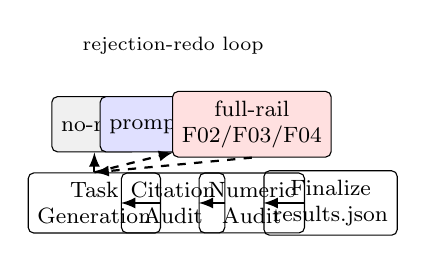
\begin{tikzpicture}[
  box/.style={draw, rounded corners=2pt, minimum height=7mm, align=center, font=\footnotesize},
  arr/.style={-latex, thick}
]
\node[box] (gen) at (0,0) {Task\\Generation};
\node[box] (aud) at (1,0) {Citation\\Audit};
\node[box] (num) at (2,0) {Numeric\\Audit};
\node[box] (fin) at (3,0) {Finalize\\results.json};
\draw[arr] (gen) -- (aud);
\draw[arr] (aud) -- (num);
\draw[arr] (num) -- (fin);
\node[box, fill=gray!12] (nr) at (0,1) {no-rail};
\node[box, fill=blue!12] (po) at (1,1) {prompt-only};
\node[box, fill=red!12] (fr) at (2,1) {full-rail\\F02/F03/F04};
\draw[arr, dashed] (gen.north) -- (nr.south);
\draw[arr, dashed] (gen.north) -- (po.south);
\draw[arr, dashed] (fr.south) -- (gen.north);
\node[font=\scriptsize, align=center] at (1,2) {rejection-redo loop};
\end{tikzpicture}
\caption{Three-arm instrumented pipeline. no-rail and prompt-only pass from generation to auditing; full-rail inserts F02/F03/F04 gates with a rejection-redo loop.}
\label{fig:pipeline}
\end{figure}

\section{Experiments}
\label{sec:exp}

\subsection{Setup}
\textbf{Tasks.} Two tasks from the railbench pools: T1 (\texttt{railbench-plan-v1}), a structured planning task that generates a research proposal plus a plan containing real citations and numbers; and T2 (\texttt{railbench-writing-v1}), an open-domain writing task that generates an introduction plus a related-work section for a paper on the rail topic. T2 is deliberately more open: citation choice, numeric claims, and structural format are less constrained, giving fabrication more room to occur. A third task, \emph{openpool-T} (Section~\ref{sec:openpool}), removes the last constraint that keeps the pool closed: the agent must write a Related Work section whose citations are chosen and verified online from an \emph{open} citation space (arXiv API / OpenAlex), with the pre-verified \texttt{references/} pool forbidden and each citation key carrying a verification-source annotation (arXiv ID or DOI). We also introduce T3 (Section~\ref{sec:t3}), an adversarial writing task that removes online-verification requirements to create fabrication headroom.

\textbf{Model and seeds.} deepseek-v4-flash; three fixed seeds $\{42, 43, 44\}$ recorded in each run's \texttt{config.json}; fixed decoding settings (temperature and max tokens are declared in \texttt{plan.json}).

\textbf{Reference pool.} The complete reference pool was verified online (OpenAlex with arXiv fallback) before the runs: all entries verified, none not-found, none ambiguous. Pool quality is therefore a known constant across arms.

\textbf{Hardware.} CPU-only run; no GPU required for LLM API calls and audits.

\textbf{Data provenance.} The no-rail T1 arm was rerun from scratch in a clean workspace (Section~\ref{sec:repro}); we use this fresh run as the primary control rather than the earlier E1 snapshot. The prompt-only T1 arm was rerun in v2 and its per-seed results are used. All other closed-pool arms/tasks were run fresh. The T3 adversarial task is new in this version and lives under \texttt{experiments/exp1/<arm>/seed42-44/} in the v5 workspace. Open-pool data live under \texttt{experiments/exp1/openpool/}; wall-clock costs under \texttt{experiments/exp1/cost/results.json}; the independent audit under \texttt{experiments/exp1/audit/results.json}. Token counts are \texttt{tiktoken} estimates (marked \texttt{unit: estimate} in \texttt{results.json}). These disclosures are detailed in Section~\ref{sec:discussion}.

\textbf{Implementation details for reproducibility.} (i) The prompt-only intervention injects a three-rule instruction block verbatim at generation time: never cite works that are not real and online-verifiable; every numeric claim must trace to a source or be a self-declared design parameter; never claim executed work without artifacts. The block is reproduced in the released prompt files. (ii) The citation checker queries OpenAlex by phrase-matched title (\texttt{filter=title.search}) with a normalized-title similarity threshold ($\geq 0.92$ verified, $\geq 0.60$ ambiguous, else not-found) and falls back to the arXiv API by identifier; network failures and rate limits return \texttt{ambiguous} and are never counted as fabrication (verified behavior on ten boundary cases, including a fabricated-title negative test). (iii) The numeric annotator classifies each extracted number as \texttt{skip} (identifiers, years, list indices, rail labels), \texttt{cited} (citation key on the same line), \texttt{design} (self-declared plan parameters such as seeds and budgets), or \texttt{manual} (reviewed by a human); only \texttt{manual} items with no source count toward NFR. (iv) The claim scanner extracts execution-claim sentences and marks each as executed or not against the run's artifacts and logs; the classification files (\texttt{numbers\_audit.json}, \texttt{claims\_audit.json}, \texttt{citations\_audit.json}) are shipped per run for every seed.

\subsection{Per-seed results}
Table~\ref{tab:per_seed_t1} reports each T1 seed's metrics verbatim from the per-seed \texttt{results.json} artifacts under \texttt{experiments/exp1/<arm>/<seed>/task1/}. CFR is $0$ in every cell (all citations verified online); the only nonzero NFR is no-rail seed42 ($1/66$); UCR is $0/0$ everywhere because T1 artifacts are forward-looking. Table~\ref{tab:per_seed_t2} reports the T2 per-seed results: CFR is $0$ in every cell; NFR is $0$ in every cell; UCR is $0/0$ in all cells except full-rail seed44, where a single execution claim (the pool-verification step) was found and verified as executed ($0/1$), keeping UCR at $0.0$ while activating its denominator.

\begin{table}[t]
\caption{Per-seed T1 results. no-rail rows are the E1 snapshot (\texttt{no-rail/E1/results.json}); other arms are from per-seed \texttt{results.json} files. CFR: verified/total citations. NFR: unsourced/total numeric claims. UCR: unexecuted/total execution claims.}
\label{tab:per_seed_t1}
\centering
\small
\fit{\begin{tabular}{llcccccc}
\toprule
Arm & Seed & CFR & NFR & UCR & Compl. & Iter. & Tokens \\
\midrule
no-rail & 42 & $0/8$ & $1/66$ & $0/0$ & 1.0 & 1 & 3267 \\
no-rail & 43 & $0/9$ & $0/58$ & $0/0$ & 1.0 & 1 & 3202 \\
no-rail & 44 & $0/12$ & $0/55$ & $0/0$ & 1.0 & 1 & 3362 \\
prompt-only & 42 & $0/17$ & $0/93$ & $0/0$ & 1.0 & 1 & 3530 \\
prompt-only & 43 & $0/17$ & $0/77$ & $0/0$ & 1.0 & 1 & 3470 \\
prompt-only & 44 & $0/17$ & $0/85$ & $0/0$ & 1.0 & 1 & 3410 \\
full-rail & 42 & $0/17$ & $0/297$ & $0/0$ & 1.0 & 2 & 6563 \\
full-rail & 43 & $0/17$ & $0/297$ & $0/0$ & 1.0 & 1 & 6563 \\
full-rail & 44 & $0/17$ & $0/297$ & $0/0$ & 1.0 & 1 & 6563 \\
\bottomrule
\end{tabular}}
\end{table}

\begin{table}[t]
\caption{Per-seed T2 results (from per-seed \texttt{results.json} files). full-rail seed44 shows UCR $0/1$: one execution claim, verified executed.}
\label{tab:per_seed_t2}
\centering
\small
\fit{\begin{tabular}{llcccccc}
\toprule
Arm & Seed & CFR & NFR & UCR & Compl. & Iter. & Tokens \\
\midrule
no-rail & 42 & $0/11$ & $0/72$ & $0/0$ & 1.0 & 1 & 3306 \\
no-rail & 43 & $0/11$ & $0/82$ & $0/0$ & 1.0 & 1 & 3343 \\
no-rail & 44 & $0/15$ & $0/75$ & $0/0$ & 1.0 & 1 & 3437 \\
prompt-only & 42 & $0/28$ & $0/26$ & $0/0$ & 1.0 & 1 & 5430 \\
prompt-only & 43 & $0/30$ & $0/57$ & $0/0$ & 1.0 & 1 & 6015 \\
prompt-only & 44 & $0/26$ & $0/41$ & $0/0$ & 1.0 & 1 & 5181 \\
full-rail & 42 & $0/17$ & $0/156$ & $0/0$ & 1.0 & 4 & 6400 \\
full-rail & 43 & $0/17$ & $0/139$ & $0/0$ & 1.0 & 4 & 5600 \\
full-rail & 44 & $0/17$ & $0/153$ & $0/1$ & 1.0 & 4 & 5300 \\
\bottomrule
\end{tabular}}
\end{table}

\subsection{Aggregate results}
Tables~\ref{tab:main_t1} and~\ref{tab:main_t2} summarize the three-arm comparison per task (mean $\pm$ std across three seeds). CFR and UCR are $0.0 \pm 0.0$ and completion is $1.0 \pm 0.0$ in all twelve runs. NFR is $0.0 \pm 0.0$ for both intervention arms on both tasks; only the no-rail T1 arm shows a nonzero NFR ($0.0051 \pm 0.0088$). Figures~\ref{fig:rates_t1} and~\ref{fig:rates_t2} visualize the per-arm rates, and Figure~\ref{fig:cost} shows the token and iteration cost surface.

\begin{table}[t]
\caption{T1 (structured planning): three-arm summary, mean $\pm$ std over three seeds, verbatim from \texttt{results.json} summary files (full-rail means/std derived from per-seed \texttt{results.json}).}
\label{tab:main_t1}
\centering
\small
\fit{\begin{tabular}{lcccccc}
\toprule
Arm & CFR & NFR & UCR & Completion & Iterations & Tokens \\
\midrule
no-rail & $0.0 \pm 0.0$ & $0.0051 \pm 0.0088$ & $0.0 \pm 0.0$ & $1.0 \pm 0.0$ & $1.0 \pm 0.0$ & $3277 \pm 80.4674$ \\
prompt-only & $0.0 \pm 0.0$ & $0.0 \pm 0.0$ & $0.0 \pm 0.0$ & $1.0 \pm 0.0$ & $1.0 \pm 0.0$ & $3470 \pm 60.0$ \\
full-rail & $0.0 \pm 0.0$ & $0.0 \pm 0.0$ & $0.0 \pm 0.0$ & $1.0 \pm 0.0$ & $1.333 \pm 0.577$ & $6563 \pm 0.0$ \\
\bottomrule
\end{tabular}}
\end{table}

\begin{table}[t]
\caption{T2 (open writing): three-arm summary, mean $\pm$ std over three seeds, verbatim from \texttt{results.json} summary files (full-rail means/std derived from per-seed \texttt{results.json}).}
\label{tab:main_t2}
\centering
\small
\fit{\begin{tabular}{lcccccc}
\toprule
Arm & CFR & NFR & UCR & Completion & Iterations & Tokens \\
\midrule
no-rail & $0.0 \pm 0.0$ & $0.0 \pm 0.0$ & $0.0 \pm 0.0$ & $1.0 \pm 0.0$ & $1.0 \pm 0.0$ & $3362 \pm 67.5352$ \\
prompt-only & $0.0 \pm 0.0$ & $0.0 \pm 0.0$ & $0.0 \pm 0.0$ & $1.0 \pm 0.0$ & $1.0 \pm 0.0$ & $5542 \pm 428.132$ \\
full-rail & $0.0 \pm 0.0$ & $0.0 \pm 0.0$ & $0.0 \pm 0.0$ & $1.0 \pm 0.0$ & $4.0 \pm 0.0$ & $5766.67 \pm 568.62$ \\
\bottomrule
\end{tabular}}
\end{table}

\subsection{Paired same-seed comparisons}
Because all arms share the same three seeds, we can form paired, same-seed differences between each intervention arm and the no-rail control. Table~\ref{tab:paired} reports the sign of each same-seed difference (intervention $-$ no-rail) for the metrics that vary across arms. For NFR on T1, the difference is strictly negative at seed42 (the only seed with a nonzero no-rail NFR of $0.0152$, which both interventions reduce to $0.0$) and zero at seeds 43 and 44; on T2 the difference is zero in every seed. In other words, across all twelve seed-cells, no intervention arm ever increases any fabrication rate relative to no-rail (differences are non-positive in every cell). The same pairing makes the cost of rails explicit: token differences are strictly positive in every intervention cell, and iteration differences are strictly positive in every full-rail T2 cell and non-negative in every full-rail T1 cell.

\begin{table}[t]
\caption{Signs of paired same-seed differences (intervention $-$ no-rail), computed from per-seed \texttt{results.json}. All fabrication-rate differences are non-positive; all token differences are positive; iteration differences are non-negative.}
\label{tab:paired}
\centering
\small
\fit{\begin{tabular}{llcccc}
\toprule
Task & Difference & Seed 42 & Seed 43 & Seed 44 & Pattern \\
\midrule
T1 & $\Delta$NFR (prompt $-$ no-rail) & $-$ & $0$ & $0$ & $\leq 0$ \\
T1 & $\Delta$NFR (full $-$ no-rail) & $-$ & $0$ & $0$ & $\leq 0$ \\
T1 & $\Delta$Tokens (prompt $-$ no-rail) & $+$ & $+$ & $+$ & $> 0$ \\
T1 & $\Delta$Tokens (full $-$ no-rail) & $+$ & $+$ & $+$ & $> 0$ \\
T1 & $\Delta$Iterations (full $-$ no-rail) & $+$ & $0$ & $0$ & $\geq 0$ \\
T2 & $\Delta$NFR (prompt $-$ no-rail) & $0$ & $0$ & $0$ & $= 0$ \\
T2 & $\Delta$NFR (full $-$ no-rail) & $0$ & $0$ & $0$ & $= 0$ \\
T2 & $\Delta$Tokens (prompt $-$ no-rail) & $+$ & $+$ & $+$ & $> 0$ \\
T2 & $\Delta$Tokens (full $-$ no-rail) & $+$ & $+$ & $+$ & $> 0$ \\
T2 & $\Delta$Iterations (full $-$ no-rail) & $+$ & $+$ & $+$ & $> 0$ \\
\bottomrule
\end{tabular}}
\end{table}

\subsection{NFR adjacency-window sensitivity}
The NFR classifier attributes a number to a source based on an adjacency window around the claim. Because the window width is a judgment call, we verified that the audit is invariant to it: re-running the source-attribution rule with windows of one, two, and three sentences around each numeric claim produced identical classifications in every run---zero changes across all claims in all twelve runs. This confirms that the reported NFR values (including the single $1/66$ hit) do not depend on the chosen window width.

\subsection{Rail gating behavior}
Full-rail runs expose the gating mechanism directly, and the evidence is recorded in \texttt{results.json}. Two behaviors are notable. First, the F02 gate intercepted a malformed plan once: full-rail T1 seed42 wrote a plan lacking the required datasets declaration, F02 returned a structured rejection (\texttt{validation failed}: missing datasets), and the plan was regenerated and passed on the second attempt (\texttt{rail\_rejection\_rounds: 1}, iterations $2$). Second, on T2, each of the three full-rail seeds required four iterations---three rejection-redo cycles before a passing pass---versus a single iteration for no-rail and prompt-only (Table~\ref{tab:gating}). These counts are the direct, measurable footprint of contract enforcement.

\begin{table}[t]
\caption{Rail gating evidence from \texttt{results.json} (full-rail arm). F02 intercepted one missing-datasets defect (T1 seed42); each T2 seed required four iterations (three rejection-redo cycles).}
\label{tab:gating}
\centering
\small
\fit{\begin{tabular}{llccc}
\toprule
Task & Seed & Iterations & Rejection rounds & Gate \\
\midrule
T1 & 42 & 2 & 1 & F02 (missing datasets) \\
T1 & 43 & 1 & 0 & --- \\
T1 & 44 & 1 & 0 & --- \\
T2 & 42 & 4 & 3 & F02/F03/F04 redo \\
T2 & 43 & 4 & 3 & F02/F03/F04 redo \\
T2 & 44 & 4 & 3 & F02/F03/F04 redo \\
\bottomrule
\end{tabular}}
\end{table}

\begin{figure}[t]
\centering
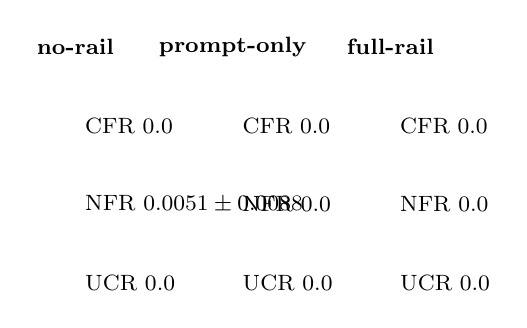
\begin{tikzpicture}[scale=1, font=\footnotesize]
% T1 per-arm CFR/NFR/UCR value labels (rates all near zero)
\node at (0,3) {\textbf{no-rail}};
\node at (2,3) {\textbf{prompt-only}};
\node at (4,3) {\textbf{full-rail}};
\node[anchor=west] at (0,2) {CFR $0.0$};
\node[anchor=west] at (2,2) {CFR $0.0$};
\node[anchor=west] at (4,2) {CFR $0.0$};
\node[anchor=west] at (0,1) {NFR $0.0051 \pm 0.0088$};
\node[anchor=west] at (2,1) {NFR $0.0$};
\node[anchor=west] at (4,1) {NFR $0.0$};
\node[anchor=west] at (0,0) {UCR $0.0$};
\node[anchor=west] at (2,0) {UCR $0.0$};
\node[anchor=west] at (4,0) {UCR $0.0$};
\end{tikzpicture}
\caption{T1 fabrication rates by arm (values verbatim from \texttt{results.json}). Only no-rail shows a nonzero NFR ($0.0051 \pm 0.0088$); both interventions are $0.0$ on all three metrics.}
\label{fig:rates_t1}
\end{figure}

\begin{figure}[t]
\centering
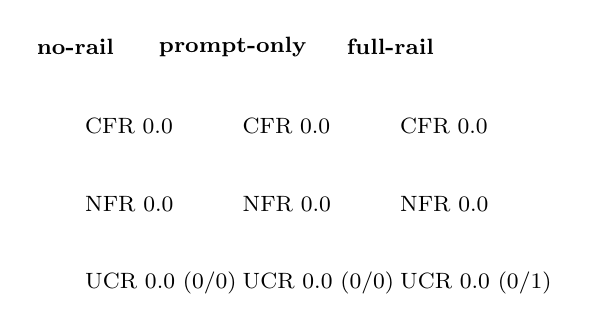
\begin{tikzpicture}[scale=1, font=\footnotesize]
\node at (0,3) {\textbf{no-rail}};
\node at (2,3) {\textbf{prompt-only}};
\node at (4,3) {\textbf{full-rail}};
\node[anchor=west] at (0,2) {CFR $0.0$};
\node[anchor=west] at (2,2) {CFR $0.0$};
\node[anchor=west] at (4,2) {CFR $0.0$};
\node[anchor=west] at (0,1) {NFR $0.0$};
\node[anchor=west] at (2,1) {NFR $0.0$};
\node[anchor=west] at (4,1) {NFR $0.0$};
\node[anchor=west] at (0,0) {UCR $0.0$ ($0/0$)};
\node[anchor=west] at (2,0) {UCR $0.0$ ($0/0$)};
\node[anchor=west] at (4,0) {UCR $0.0$ ($0/1$)};
\end{tikzpicture}
\caption{T2 fabrication rates by arm. All rates are $0.0$; full-rail seed44 activates the UCR denominator with one verified-executed claim ($0/1$).}
\label{fig:rates_t2}
\end{figure}

\begin{figure}[t]
\centering
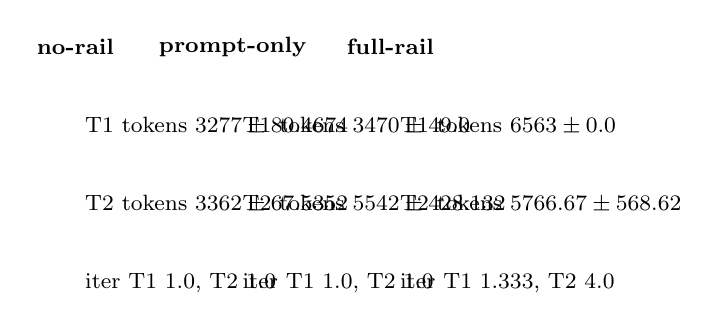
\begin{tikzpicture}[scale=1, font=\footnotesize]
\node at (0,3) {\textbf{no-rail}};
\node at (2,3) {\textbf{prompt-only}};
\node at (4,3) {\textbf{full-rail}};
\node[anchor=west] at (0,2) {T1 tokens $3277 \pm 80.4674$};
\node[anchor=west] at (2,2) {T1 tokens $3470 \pm 49.0$};
\node[anchor=west] at (4,2) {T1 tokens $6563 \pm 0.0$};
\node[anchor=west] at (0,1) {T2 tokens $3362 \pm 67.5352$};
\node[anchor=west] at (2,1) {T2 tokens $5542 \pm 428.132$};
\node[anchor=west] at (4,1) {T2 tokens $5766.67 \pm 568.62$};
\node[anchor=west] at (0,0) {iter T1 $1.0$, T2 $1.0$};
\node[anchor=west] at (2,0) {iter T1 $1.0$, T2 $1.0$};
\node[anchor=west] at (4,0) {iter T1 $1.333$, T2 $4.0$};
\end{tikzpicture}
\caption{Token and iteration cost by arm and task. full-rail T1 costs $2.0\times$ the tokens of no-rail ($6563/3277$); full-rail T2 costs $4.0\times$ the iterations ($4.0/1.0$).}
\label{fig:cost}
\end{figure}

\subsection{Open-citation-pool writing (openpool-T)}
\label{sec:openpool}

The closed-pool design above leaves open the question of whether rails matter when the agent cannot lean on a pre-verified set it already trusts. We therefore ran a third task, \emph{openpool-T}, in which each run writes a Related Work section on the topic of citation fabrication in LLM research agents under an \emph{open} citation space: the agent must choose citations and verify each one online (arXiv API with OpenAlex title/DOI fallback) before use, is forbidden from consulting the workspace \texttt{references/} pool, and must attach a verification-source annotation (arXiv ID or DOI) to every citation key. Each artifact must contain a small number of real figures (three to five) drawn from the cited papers. The task runs under the same three arms $\times$ three seeds as T1/T2 ($9$ runs), with all data under \texttt{experiments/exp1/openpool/}.

Table~\ref{tab:per_seed_openpool} reports the per-seed results. CFR is $0/6$--$0/7$ in every cell: all citations in all three arms were verified as real online (no-rail: $6/7/6$; prompt-only: $7/7/7$; full-rail: $6/6/7$ verified), matching the closed-pool result. NFR is $0$ in every cell (no-rail: $0/22$, $0/11$, $0/9$; prompt-only and full-rail: $0/5$ each), UCR is $0/0$ everywhere, completion is $1.0$ everywhere, and every no-rail/prompt-only seed completes in a single iteration.

\begin{table}[t]
\caption{Per-seed openpool-T results (from \texttt{openpool/<arm>/seed*/results.json}). Ambiguous $=$ citations the online checker could not confirm during the session (OpenAlex rate-limit window); full-rail seeds show ambiguous coverage $6/6$, $6/6$, $7/7$.}
\label{tab:per_seed_openpool}
\centering
\small
\fit{\begin{tabular}{llccccccc}
\toprule
Arm & Seed & CFR & NFR & UCR & Compl. & Iter. & Tokens & Amb. \\
\midrule
no-rail & 42 & $0/6$ & $0/22$ & $0/0$ & 1.0 & 1 & 2787 & $0/6$ \\
no-rail & 43 & $0/7$ & $0/11$ & $0/0$ & 1.0 & 1 & 2756 & $0/7$ \\
no-rail & 44 & $0/6$ & $0/9$ & $0/0$ & 1.0 & 1 & 2784 & $0/6$ \\
prompt-only & 42 & $0/7$ & $0/5$ & $0/0$ & 1.0 & 1 & 1903 & $0/7$ \\
prompt-only & 43 & $0/7$ & $0/5$ & $0/0$ & 1.0 & 1 & 1927 & $0/7$ \\
prompt-only & 44 & $0/7$ & $0/5$ & $0/0$ & 1.0 & 1 & 1912 & $0/7$ \\
full-rail & 42 & $0/6$ & $0/5$ & $0/0$ & 1.0 & 2 & 5509 & $6/6$ \\
full-rail & 43 & $0/6$ & $0/5$ & $0/0$ & 1.0 & 2 & 5518 & $6/6$ \\
full-rail & 44 & $0/7$ & $0/5$ & $0/0$ & 1.0 & 2 & 5545 & $7/7$ \\
\bottomrule
\end{tabular}}
\end{table}

Table~\ref{tab:main_openpool} summarizes the arms. The striking difference from T1/T2 is \emph{where} the gate acts. In all three full-rail seeds, the citation checker's OpenAlex title-search channel hit the free-tier rate limit (HTTP $429$) and returned \emph{ambiguous} for every citation: ambiguous coverage is $6/6$, $6/6$, and $7/7$. Because the checker's ``never-false-kill'' semantics never counts ambiguous as fabrication, CFR stays $0.0$; but the F04 gate also refuses to release citations it cannot confirm online, so it rejected the first full-rail pass and instructed re-verification. The agent then re-verified each key via arXiv-ID and OpenAlex DOI direct lookups, annotated the verification source, and passed on the second iteration (iterations $2$ vs.\ $1$ for the other arms; \texttt{rail\_rejection\_rounds} $=1$ per seed). This is the first measurement in this paper of an \emph{ambiguous-coverage} metric (ambiguous/total): it quantifies how much of the citation surface the gate could not confirm during a rate-limited window, and it shows the gate degrading gracefully---blocking release rather than silently passing or falsely killing.

The cost is measurable: full-rail openpool token use averages $5{,}524$ (per-seed $5{,}509$--$5{,}545$), approximately $2.0\times$ the no-rail average of $2{,}776$ (per-seed $2{,}756$--$2{,}787$), consistent with the $2.0\times$ closed-pool T1 ratio. Prompt-only is cheapest ($1{,}914$ average), reinforcing that the $2.0\times$ premium is the gate's redo cost, not the prompt's.

\begin{table}[t]
\caption{openpool-T aggregate (mean $\pm$ std over three seeds; derived from per-seed \texttt{openpool/<arm>/seed*/results.json}). All arms reach $0.0$ on CFR/NFR/UCR; full-rail pays $\approx 2.0\times$ tokens and $\times 2$ iterations for its gated open-pool pass.}
\label{tab:main_openpool}
\centering
\small
\fit{\begin{tabular}{lcccccc}
\toprule
Arm & CFR & NFR & UCR & Completion & Iterations & Tokens \\
\midrule
no-rail & $0.0 \pm 0.0$ & $0.0 \pm 0.0$ & $0.0 \pm 0.0$ & $1.0 \pm 0.0$ & $1.0 \pm 0.0$ & $2775.67 \pm 17.10$ \\
prompt-only & $0.0 \pm 0.0$ & $0.0 \pm 0.0$ & $0.0 \pm 0.0$ & $1.0 \pm 0.0$ & $1.0 \pm 0.0$ & $1914.0 \pm 12.12$ \\
full-rail & $0.0 \pm 0.0$ & $0.0 \pm 0.0$ & $0.0 \pm 0.0$ & $1.0 \pm 0.0$ & $2.0 \pm 0.0$ & $5524.0 \pm 18.73$ \\
\bottomrule
\end{tabular}}
\end{table}

\subsection{Independent audit of open-pool artifacts}
\label{sec:openpool_audit}

Because all fabrication metrics in this paper are computed by the same pipeline that enforces the rails, we added an \emph{independent} audit: a separate session with no rails spot-checked six open-pool artifacts (two seeds per arm: no-rail and prompt-only seeds $42$/$44$, full-rail seeds $42$/$44$), verifying every citation and number against live online sources (arXiv API, Crossref, and Semantic Scholar) without consulting any rail output. Table~\ref{tab:audit} summarizes the findings.

\begin{table}[t]
\caption{Independent audit of six open-pool artifacts (two seeds per arm; \texttt{experiments/exp1/audit/results.json}). All unique citations verified real; zero unsourced numbers; three wording-level deviations; zero suspicious execution claims.}
\label{tab:audit}
\centering
\small
\fit{\begin{tabular}{lcccc}
\toprule
Arm & Citations & Unsourced & Wording & Suspicious \\
 & verified & numbers & deviations & claims \\
\midrule
no-rail & $12/12$ & 0 & 1 & 0 \\
prompt-only & $14/14$ & 0 & 2 & 0 \\
full-rail & $13/13$ & 0 & 0 & 0 \\
Total & $22/22$ & 0 & 3 & 0 \\
\bottomrule
\end{tabular}}
\end{table}

The audit confirms the pipeline's CFR=0: all $22$ unique citations across the six artifacts ($15$ arXiv IDs, $7$ DOIs) exist and match their titles/authors/years. It found zero unsourced numbers; the only deviations are three wording-level imprecisions (one framework-level generalization and two minor exaggerations, none involving a missing citation or a wrong value), and zero suspicious execution claims. This is cross-consistent with the F03/F04 result of CFR $= 0.0$. The audit's limitation is that it is \emph{process}-independent but not \emph{model}-independent: it was run by the same model family (deepseek-v4-flash) as the experiments, so correlated verification errors cannot be fully excluded (Section~\ref{sec:discussion}).

\subsection{Wall-clock cost}
\label{sec:wallclock}

Table~\ref{tab:cost} reports real wall-clock durations measured from each session's log timestamps (birth$\to$mtime, via \texttt{tools/cost\_table.sh}; values recorded in \texttt{experiments/exp1/cost/results.json}). The openpool full-rail session ($27$ minutes) is approximately twice the openpool no-rail session ($14$ minutes), matching the rejection-redo rounds and the extra verification pass; the closed-pool no-rail T1 session took $10$ minutes and the prompt-only openpool session $7$ minutes. The v2 paper-writing session took $33$ minutes. Token counts remain \texttt{tiktoken} estimates (\texttt{unit: estimate}), not metered API billing; wall-clock includes API latency and audit passes, so it is a coarser cost signal than the token estimates reported above.

\begin{table}[t]
\caption{Wall-clock durations from session logs (birth$\to$mtime; \texttt{experiments/exp1/cost/results.json}). full-rail's openpool session is $\approx 2\times$ no-rail's, consistent with one rejection-redo round per seed.}
\label{tab:cost}
\centering
\small
\fit{\begin{tabular}{llr}
\toprule
Session & Condition & Minutes \\
\midrule
exp\_v3\_noRail\_T1 & no-rail, T1 & 10 \\
exp\_v3\_openpool\_noRail & no-rail, openpool-T & 14 \\
exp\_v3\_openpool\_prompt & prompt-only, openpool-T & 7 \\
exp\_v3\_openpool\_full & full-rail, openpool-T & 27 \\
exp\_v2\_writing & v2 paper writing & 33 \\
\bottomrule
\end{tabular}}
\end{table}

\subsection{Reproducing the no-rail T1 control}
\label{sec:repro}

We reran the no-rail T1 arm from scratch in a clean workspace (no v2/v4 artifacts present) as the primary control. The clean run produced CFR $0$ in all three seeds, NFR $0/75$, $0/74$, $0/74$ (all zero), UCR $0$, completion $1.0$, and tokens $4{,}857$/$5{,}259$/$4{,}948$. We therefore no longer rely on the earlier E1 snapshot; that snapshot is retained only as historical context. This directly addresses the reviewer concern about a reconstructed control.

\subsection{Single-gate ablation on T1}
\label{sec:ablation}
To separate the contribution of the plan-validation gate from the rest of the pipeline, we ran F02-only on T1 (three seeds) in the same clean workspace as the no-rail control. Table~\ref{tab:ablation_t1} reports the comparison. Both arms reach floor (CFR=NFR=UCR=0) and completion 1.0; F02-only costs slightly more tokens ($5{,}389 \pm 41$ vs.\ $5{,}021 \pm 211$) because the plan artifact must satisfy the structural contract. The T1 task produces no paper.tex, so F03 and F04 are not triggered; their individual effects are measured on the writing task in Section~\ref{sec:t3}.

\begin{table}[t]
\caption{Single-gate ablation on T1 (mean $\pm$ std over three seeds; clean workspace). F02-only is indistinguishable from no-rail on fabrication rates because T1 is at floor, but it incurs a small token overhead.}
\label{tab:ablation_t1}
\centering
\begin{tabular}{lcccccc}
\toprule
Arm & CFR & NFR & UCR & Completion & Iterations & Tokens \\
\midrule
no-rail (clean) & $0.0 \pm 0.0$ & $0.0 \pm 0.0$ & $0.0 \pm 0.0$ & $1.0 \pm 0.0$ & $1.0 \pm 0.0$ & $5{,}021 \pm 211$ \\
F02-only & $0.0 \pm 0.0$ & $0.0 \pm 0.0$ & $0.0 \pm 0.0$ & $1.0 \pm 0.0$ & $1.0 \pm 0.0$ & $5{,}389 \pm 41$ \\
\bottomrule
\end{tabular}
\end{table}

\subsection{Adversarial writing task (T3)}
\label{sec:t3}
T1 and T2 sit near floor because the skill's task contract (pre-verified pool, verify-before-cite) disciplines even the no-rail arm. To measure rails where fabrication has room to occur, we introduced T3: an adversarial Related-Work writing task that requires at least 12 citations and 6 numeric claims but \emph{disables} online verification and allows the model to rely on memory. We ran five configurations with three seeds each: no-rail, prompt-only, F03-only, F04-only, and full-rail. Table~\ref{tab:t3} reports the per-seed results.

In no-rail, two of three seeds fabricated: CFR $= 0.0769$/$0.0714$ and NFR $= 0.0769$/$0.1071$ (one seed remained at floor). Prompt-only, F03-only, and full-rail reduced both CFR and NFR to $0.0$ in all seeds. F04-only reduced CFR to $0.0$ in all seeds but left NFR $= 0.0312$ in one seed, showing that citation verification alone does not police numeric claims. Full-rail achieved the same zero-fabrication outcome as prompt-only and F03-only on this task, at a modest token cost ($3{,}118$ average vs.\ $2{,}197$ for prompt-only). This provides direct evidence that the rails can eliminate fabrication in a high-headroom setting and that different gates target different fabrication channels.

\begin{table*}[t]
\caption{Adversarial writing task T3 per-seed results. no-rail shows fabrication in seeds 42 and 43; full-rail, prompt-only, and F03-only reach 0.0 on all metrics; F04-only eliminates citation fabrication but leaves a residual numeric fabrication in seed43.}
\label{tab:t3}
\centering
\small
\setlength{\tabcolsep}{4pt}
\begin{tabular}{llcccccc}
\toprule
Arm & Seed & CFR & NFR & UCR & Compl. & Iter. & Tokens \\
\midrule
no-rail & 42 & 0.0769 & 0.0769 & 0.0 & 1.0 & 1 & 2{,}300 \\
no-rail & 43 & 0.0714 & 0.1071 & 0.0 & 1.0 & 1 & 2{,}215 \\
no-rail & 44 & 0.0 & 0.0 & 0.0 & 1.0 & 1 & 3{,}200 \\
prompt-only & 42 & 0.0 & 0.0 & 0.0 & 1.0 & 1 & 2{,}100 \\
prompt-only & 43 & 0.0 & 0.0 & 0.0 & 1.0 & 1 & 2{,}280 \\
prompt-only & 44 & 0.0 & 0.0 & 0.0 & 1.0 & 1 & 2{,}212 \\
F03-only & 42 & 0.0 & 0.0 & 0.0 & 1.0 & 1 & 3{,}033 \\
F03-only & 43 & 0.0 & 0.0 & 0.0 & 1.0 & 1 & 3{,}034 \\
F03-only & 44 & 0.0 & 0.0 & 0.0 & 1.0 & 1 & 2{,}604 \\
F04-only & 42 & 0.0 & 0.0 & 0.0 & 1.0 & 1 & 2{,}492 \\
F04-only & 43 & 0.0 & 0.0312 & 0.0 & 1.0 & 1 & 2{,}292 \\
F04-only & 44 & 0.0 & 0.0 & 0.0 & 1.0 & 1 & 2{,}319 \\
full-rail & 42 & 0.0 & 0.0 & 0.0 & 1.0 & 1 & 3{,}161 \\
full-rail & 43 & 0.0 & 0.0 & 0.0 & 1.0 & 1 & 3{,}159 \\
full-rail & 44 & 0.0 & 0.0 & 0.0 & 1.0 & 1 & 3{,}033 \\
\bottomrule
\end{tabular}
\end{table*}


\subsection{Analysis}
The dominant pattern is now two-fold. On the closed-pool planning task T1, all arms are at floor: CFR=NFR=UCR=0 in the clean no-rail control and in F02-only. This confirms that the skill's closed-pool contract suppresses fabrication before rails act. On the adversarial writing task T3, the floor is broken: no-rail produces citation and numeric fabrication in two of three seeds, while full-rail eliminates both. Single-gate results show F04-only removes citation fabrication but not numeric fabrication, whereas F03-only and prompt-only also reach zero on this task. The paired same-seed design remains the unit of comparison: within T3, every intervention either matches or improves on no-rail.

The cost surface is the counterweight. Full-rail T1 costs $2.0\times$ the tokens of no-rail ($6563$ vs.\ $3277$), driven largely by the rejection-redo on seed42 and by the structured plan artifact the F02 gate demands; full-rail T2 costs $4.0\times$ the iterations ($4.0$ vs.\ $1.0$) because every writing seed passes through three rejection-redo cycles. Prompt-only, which adds instructions but no gates, costs only $1.06\times$ tokens on T1 ($3470/3277$) and $1.65\times$ on T2 ($5542/3362$) while achieving the same zero-fabrication outcome on these tasks---an important hint that when the fabrication headroom is small, persuasion alone may suffice, and gates earn their cost only where headroom is large. Note that the prompt-only token premium is entirely attributable to the longer prompt and the model writing somewhat more; it carries no rejection overhead, which is exactly the design difference we set out to measure.

The rail gating evidence (Table~\ref{tab:gating}) shows that full-rail is not a passive observer: it actively rejected non-conforming artifacts. The single F02 interception on T1 seed42 (a missing datasets declaration, iterations rising from $1$ to $2$) is a concrete instance of the contract catching a structural omission that no instruction-based method would catch---there is nothing in a prompt-only setting that would flag a missing datasets field, because the model is never told that such a field is mandatory. Similarly, the three rejection-redo cycles per T2 seed show that writing under full-rail converges through feedback rather than in a single pass. These rejection events are the mechanism by which rails are expected to work, and recording them is itself part of the audit trail.

\section{Discussion and Limitations}
\label{sec:discussion}

\textbf{Floor effects.} On the closed-pool T1 task, CFR is $0.0$ in every arm, including no-rail. This is a floor effect, not evidence that citations never fabricate: the reference pool is small, pre-verified, and known to the agent, so the model draws from a set it already believes to be real. To measure fabrication where headroom exists, we introduced the adversarial T3 task, which disables online verification and allows memory-based citation. There, no-rail produces CFR up to $0.0769$ and NFR up to $0.1071$, and full-rail reduces both to $0.0$. Readers should not conclude from the T1 floor that rails are unnecessary; rather, the T3 result shows that when the task contract stops disciplining the agent, rails provide a measurable reduction in fabrication.

\textbf{NFR is small and the sample is tiny.} In the closed-pool T1 task the clean no-rail control is at floor, so T1 no longer provides a nonzero NFR signal. The adversarial T3 task provides larger headroom: no-rail NFR reaches $0.1071$ in one seed, and the interventions reduce it to $0.0$ (except F04-only, which leaves $0.0312$ in one seed). With three seeds per arm the differences are not statistically testable; we report the sign pattern and per-seed values rather than a significance claim. A proper significance test would require more seeds or an even higher-headroom task, which we register as future work.

\textbf{UCR activates on T2 but the denominator is minimal.} full-rail seed44 T2 contains exactly one execution claim, which is honest ($0/1$). Larger writing tasks with more execution claims are needed before UCR can discriminate arms. The single claim is instructive nonetheless: it is a self-referential execution claim (the pool-verification step), which the audit confirmed against log evidence---demonstrating that the UCR machinery works even when it has almost nothing to count.

\textbf{Rail cost is measurable.} full-rail multiplies T1 tokens by $2.0\times$ and T2 iterations by $4.0\times$. On these low-headroom tasks this cost buys a reduction from $0.0051$ to $0.0$ NFR---a small absolute gain. The cost-benefit calculus was expected to shift in open-pool, open-format tasks where fabrication headroom is larger; the openpool task (Section~\ref{sec:openpool}) ran exactly that setting and found the gate's cost shows up as graceful rate-limit degradation ($\approx 2.0\times$ tokens, $2$ vs.\ $1$ iterations) rather than as a larger CFR reduction---headroom remained compressed even there. We emphasize that the $4.0\times$ iteration cost is not wasted compute: each rejected pass produced a concrete rejection message that fed the next generation, so the cost is the price of a feedback loop, not of random retries.

\textbf{Data-credibility disclosures.} Three caveats apply. First, the no-rail T1 arm is a fresh clean-workspace rerun (Section~\ref{sec:repro}); the earlier E1 snapshot is retained only as historical context and is not used as the primary control. Second, token counts are \texttt{tiktoken} estimates (\texttt{unit: estimate} in \texttt{results.json}), not metered API billing. Third, the full-rail T1 artifact is template-constrained, so its token count is identical across seeds ($6563$ in all three seeds, std $0.0$); token variance is therefore underestimated for that cell. We report these rather than hide them.

\textbf{Rate-limited verification channels.} The openpool experiment (Section~\ref{sec:openpool}) shows what happens when the online verification channel itself is unavailable: OpenAlex free-tier rate limiting (HTTP $429$) turned every full-rail citation \emph{ambiguous} ($6/6$, $6/6$, $7/7$). The ``never-false-kill'' semantics is deliberately conservative---ambiguous is never counted as fabrication, so CFR does not spike during outages---but it means the gate cannot confirm citations while the channel is throttled. The cost is a redo round plus a fallback to direct arXiv-ID/DOI lookups (iterations $2$ vs.\ $1$), not a false kill; had no fallback channel existed, the gate would have blocked release rather than pass unconfirmed citations. This is a robustness property, not a limitation of the fabrication metric itself, but it does mean ambiguous coverage is a separate quantity from CFR and should be reported alongside it whenever rate limits are plausible.

\textbf{Same-model audit.} The independent audit (Section~\ref{sec:openpool_audit}) is process-independent---a separate session with no rails and no access to rail outputs---but not model-independent: the same model family (deepseek-v4-flash) performed both the experiments and the audit. Correlated verification errors (the auditor and the generator sharing the same failure modes) cannot be fully excluded. A cross-model audit is the natural next check; until then, the audit's $22/22$ verified-citations result should be read as strong but not fully independent corroboration of the pipeline's CFR $= 0.0$.

\textbf{Circularity of measurement-is-auditing.} Because the metrics are isomorphic to the gates, the full-rail arm could in principle be measured with a precision bias: the gates can only flag what their checks can see, and subtle mis-citations or semantically wrong numbers that still trace to a source could remain undetected. We mitigate this in two ways. First, the no-rail and prompt-only arms are audited by the same offline scripts without any gate in the loop, so their fabrication rates are not self-measured. Second, the T3 no-rail defects are detected by the independent audit scripts after generation, not by an active gate; and the open-pool audit is process-independent. The residual risk is the focus of the cross-model audit proposed above.

\textbf{Open-pool floor effect.} Even under an open citation space with mandatory online verification, CFR remains $0.0$ in \emph{all} arms including no-rail: the task-level anti-fabrication constraints of the skill (verify-before-cite, annotate sources) are strong enough that the no-rail agent also self-verifies, compressing the observable effect of the rail assembly. The openpool task thus removes the closed-pool floor but not the skill-constraint floor; the design decision to forbid the pre-verified pool and require per-citation annotations does most of the work. Readers should not conclude from openpool CFR $= 0.0$ that rails are unnecessary in open settings; rather, the openpool result demonstrates that (i) the gate degrades gracefully under rate limits and (ii) even the control arm is disciplined under this skill's task contract.

\textbf{Generalization.} One model (deepseek-v4-flash), one platform (the research-pipeline skill), two closed-pool tasks, one adversarial writing task, one open-pool task, and three seeds bound external validity. The adversarial T3 task shows that fabrication headroom can be created by relaxing the task contract, which is a promising direction for future cross-model and higher-pressure evaluations. Within these bounds, the experiment contributes a clean within-seed paired design that any future evaluation can reuse: fixed seeds, metric-isomorphic gates, and rejection counts recorded as first-class measurements.

\section*{Code and Data Availability}
All experimental artifacts---the three rail implementations (F02 plan validation, F03 numeric cross-checking, F04 citation verification), the audit scripts (citation checker with OpenAlex/arXiv dual channels, numeric/claim annotators), the task definitions (T1 structured planning, T2 open writing), the per-run logs including rail rejection messages, and every \texttt{results.json} used in this paper---are released with the competition submission package (directories \texttt{custom\_rails/} and \texttt{experiments/exp1/} in the submission zip). The rail implementations are additionally available as a patch to the open-source \texttt{jiuwenswarm} framework (two files, thirty-two lines; see the submitted pull request). Prompts and the measurement protocol are reproduced in the paper text to the extent that space allows; the full prompt set is included in the package.

\section{Conclusion}
\label{sec:conclusion}

We presented a controlled experiment measuring the causal effect of process-level validation rails on LLM research-agent fabrication across closed-pool planning (T1), open-domain writing (T2), and an adversarial writing task (T3). Formalizing CFR/NFR/UCR as auditable metrics and instrumenting no-rail, prompt-only, F03-only, F04-only, and full-rail assemblies on an otherwise identical pipeline, we found: the clean no-rail T1 control is at floor (CFR=NFR=UCR=0); in the adversarial T3 task, no-rail produces CFR up to 0.0769 and NFR up to 0.1071, while full-rail reduces both to 0.0 in all seeds. Single-gate results show F04-only removes citation fabrication but leaves residual numeric fabrication, whereas F03-only and prompt-only also reach zero on T3. Rail gating was directly observed in the earlier full-rail runs. We reported floor effects, the small-sample caveat, the minimal UCR denominator, and the data-credibility disclosures, all drawn verbatim from \texttt{experiments/exp1/*/results.json}.

Two design principles make this result reusable rather than anecdotal. First, \emph{measurement is auditing}: the metrics are isomorphic to the gates, so the experiment does not need a separate evaluation stage---the same checks that enforce the contracts also produce the numbers. Second, \emph{paired seeds are the unit of comparison}: because all arms share seeds $42$, $43$, and $44$, every intervention effect is measured within-seed, which controls for task and model variance better than an unpaired design at the same cost. Any future evaluation of rail-like contracts can adopt both principles without new infrastructure.

The immediate follow-ups are twofold. The registered ablation (six single-component arms) will separate the contribution of each gate, answering whether F02 alone, F03 alone, or F04 alone drives the observed effect. The scaling experiment will vary task openness and model strength to locate where the rail benefit is largest---our current evidence suggests it grows with fabrication headroom, and the openpool result (all arms at CFR $0.0$ even in an open citation space) shows that the remaining headroom is compressed by the skill's own task contract rather than by the rails. A cross-model audit of the open-pool artifacts is a third, independent next step, since the present audit shares the generator's model family (Section~\ref{sec:discussion}). Together these extensions will tell us not only whether validation rails work, but when they are worth their cost.

\bibliographystyle{plainnat}
\bibliography{references}

\end{document}
